\subsection{Benchmarking} \label{results:benchmarking}
In order to benchmark the effectiveness of the added GPU acceleration in GKAGE, we decided to benchmark GKAGE against KAGE to account for the speedup.
The choice of only benchmarking GKAGE against KAGE was made based on the fact that KAGE recently showed that it was an order of magnitude faster than any other known genotyper \cite{kage}.

\subsubsection{Snakemake pipeline}
In order to adequately benchmark GKAGE, we set up a Snakemake pipeline that runs both KAGE and GKAGE on a full human genome and records the runtimes while also checking that the results of both processes are identical.
This Snakemake pipeline can be found at \url{https://github.com/kage-genotyper/GKAGE-benchmarking}.

\subsubsection{Systems}
We benchmarked GKAGE against KAGE on two systems.
\textbf{System 1}: a high-end compute server with a 64-core AMD EPYC 7742 CPU and two Nvidia Tesla V100 GPUs.
\textbf{System 2}: a consumer grade desktop with a 6-core Intel Core i5-11400F CPU and a Nvidia GTX 1660 SUPER GPU.

\vspace{1em}
\begin{table}[H]
\begin{center}
\begin{tabular}{lllll}
\cline{1-3}
\multicolumn{1}{|l|}{\textbf{System}} & \multicolumn{1}{l|}{\textbf{CPU}}                  & \multicolumn{1}{l|}{\textbf{GPU}}                   &  \\ \cline{1-3}
\multicolumn{1}{|l|}{1: High-end server} & \multicolumn{1}{l|}{AMD EPYC 7742}        & \multicolumn{1}{l|}{2x Nvidia Tesla V100}     &  \\ \cline{1-3}
\multicolumn{1}{|l|}{2: Consumer desktop} & \multicolumn{1}{l|}{Intel Core i5-11400F} & \multicolumn{1}{l|}{Nvidia GTX 1660 SUPER} &  \\ \cline{1-3}
\end{tabular}
\end{center}
\caption{
  The two systems used to benchmark GKAGE against KAGE to account for the speedup achieved through GPU acceleration.
  \textbf{System 1} is a high-end compute server with top-of-the-line hardware.
  \textbf{System 2} is a consumer grade desktop gaming computer.
}
\label{results:gkage:tables:systems}
\end{table}

Benchmarking on these two systems allowed us to benchmark GKAGE on both a very performant and a less performant system to examine the effects of GPU acceleration in both instances.
A caveat with the high-end server system (system 1) was that it was it was a publicly available server for students at the University of Oslo.
Thus, students were frequently running jobs on the server, occupying both CPU and GPU processing cores and memory.
To the best of our capacity, we conducted our benchmarking during periods of lower activity.

\subsubsection{Runtimes}
We benchmarked GKAGE against KAGE on both system 1 and system 2.
When running on system 1, we allowed KAGE 16 cores and GKAGE one Nvidia Tesla V100 GPU.
When running on system 2, we allowed KAGE 6 cores and GKAGE the Nvidia GTX 1660 SUPER GPU.
We ran the Snakemake pipeline, benchmarking GKAGE against KAGE, on both systems and achieved the following results:

\begin{table}[H]
\begin{center}
\begin{tabular}{lllll}
\multicolumn{1}{l|}{System} & \multicolumn{1}{l}{KAGE}     & \multicolumn{1}{l}{GKAGE} &  \\ \cline{1-3}
\multicolumn{1}{l|}{1}      & \multicolumn{1}{l}{1993 sec} & \multicolumn{1}{l}{178 sec} &  \\
\multicolumn{1}{l|}{2}      & \multicolumn{1}{l}{510 sec}  & \multicolumn{1}{l}{94 sec} &  \\
\end{tabular}
\end{center}
\caption{
  The resulting runtimes (in seconds) found by benchmarking GKAGE against KAGE on a high-end server and a consumer desktop computer
}
\label{results:benchmarking:tables:runtimes}
\end{table}

\begin{figure}[H]
\hspace*{3em}
\begin{subfigure}{.4\textwidth}
  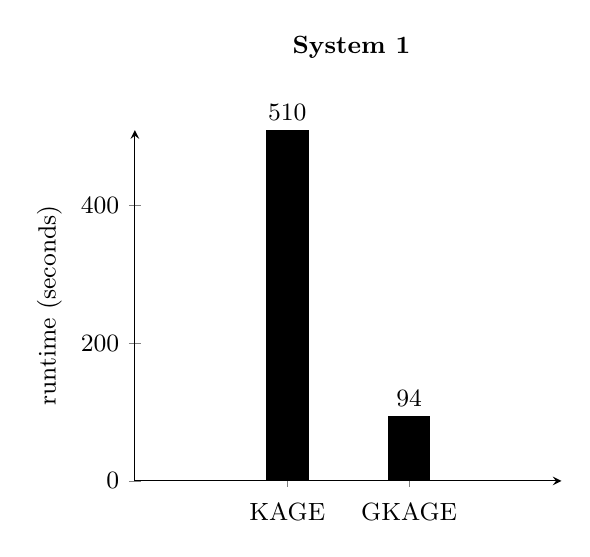
\begin{tikzpicture}[font=\small]
    \pgfplotsset{
      compat=newest,
      xlabel near ticks,
      ylabel near ticks
    }
    \pgfplotsset{compat=1.11,
        /pgfplots/ybar legend/.style={
        /pgfplots/legend image code/.code={%
           \draw[##1,/tikz/.cd,yshift=-0.25em]
            (0cm,0cm) rectangle (3pt,0.8em);},
       },
    }
    \node at(2.75,5.5)(title){\textbf{System 1}};
 
\begin{axis} [
  ylabel={runtime (seconds)},
  width=7cm,
  ybar,
  bar width=15pt,
  ymin=0,
  xtick=data,
  axis x line=bottom,
  axis y line=left,
  enlarge x limits=1.25,
  symbolic x coords={KAGE, GKAGE},
  xticklabel style={anchor=base, yshift=-\baselineskip},
  /pgf/number format/.cd,fixed,precision=3,
  nodes near coords={\small\pgfmathprintnumber{\pgfplotspointmeta}},
  legend style={anchor=west},
]

\addplot[fill=black] coordinates {
    (KAGE, 510)
    (GKAGE, 94)
};
\end{axis}

\end{tikzpicture}
\end{subfigure}
\begin{subfigure}{.4\textwidth}
  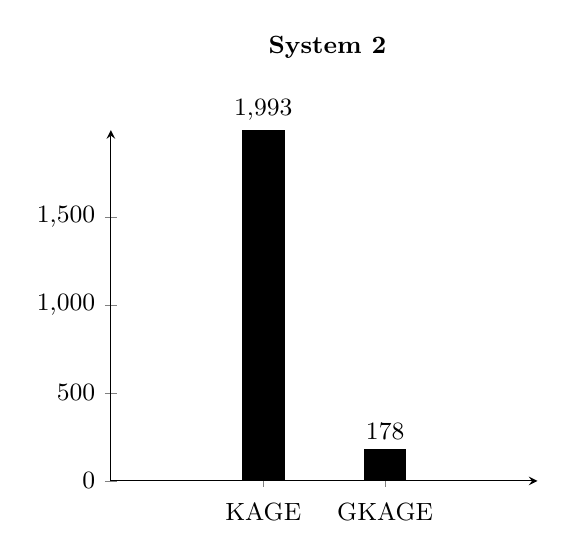
\begin{tikzpicture}[font=\small]
    \pgfplotsset{
      compat=newest,
      xlabel near ticks,
      ylabel near ticks
    }
    \pgfplotsset{compat=1.11,
        /pgfplots/ybar legend/.style={
        /pgfplots/legend image code/.code={%
           \draw[##1,/tikz/.cd,yshift=-0.25em]
            (0cm,0cm) rectangle (3pt,0.8em);},
       },
    }
    \node at(2.75,5.5)(title){\textbf{System 2}};
 
\begin{axis} [
  width=7cm,
  ybar,
  bar width=15pt,
  ymin=0,
  xtick=data,
  axis x line=bottom,
  axis y line=left,
  enlarge x limits=1.25,
  symbolic x coords={KAGE, GKAGE},
  xticklabel style={anchor=base, yshift=-\baselineskip},
  /pgf/number format/.cd,fixed,precision=3,
  nodes near coords={\small\pgfmathprintnumber{\pgfplotspointmeta}},
  legend style={anchor=west},
]

\addplot[fill=black] coordinates {
    (KAGE, 1993)
    (GKAGE, 178)
};
\end{axis}
\end{tikzpicture}
\end{subfigure}
\caption{
  Benchmarking GKAGE against KAGE on both system 1 (high-end server) and system 2 (consumer desktop) revealed that GKAGE could genotype a full human genome more than 5 times faster than KAGE on a high-end server, and more than 11 times faster on a consumer desktop computer.
}
\label{results:benchmarking:figures:runtimes}
\end{figure}

The results from the benchmarking revealed that GKAGE achieves significant speedup over KAGE when genotyping a full human genome.
As seen in table \ref{results:benchmarking:tables:runtimes} and figure \ref{results:benchmarking:figures:runtimes}, we can see that GKAGE achieves more than 5X speedup over KAGE on a high-end compute server and more than 11X speedup on a consumer grade desktop computer.
